\chapter{Surrogate Architecture}
\label{ch:architecture}

% ---------------------------------------------------------------------------
% Numbers in this chapter that depend on the training corpus (data/v2, Ch. 7).
% Update these, not the arguments, after a corpus rebuild. Source for all of
% them: SURROGATE_FORMULATION_NOTE.md and scripts/measure_formulation.py on
% branch surrogate-gns.
%   - tab:arch_anchor_velocity, tab:arch_anchor_position, fig:arch_anchor
%   - tab:arch_stiffness (omega from 60 sampled consists), omega*h = 7.45
%   - couplers outside the slack 91.1% of the time
%   - tab:arch_position_split (trapezoid errors)
%   - peak-force aliasing check: 0.4% median, 3.7% worst of 6
%   - float32 quantization: std 0.753 mm, ratios 0.77 and 117,713
%   - actuator check: 3.6e-3 N on 9.2e4 N
%   - wave speed 167-193 m/s
% Corpus-independent: the zero-residual argument, the 50-evaluation ratio,
% the parameter count, the network structure.
% ---------------------------------------------------------------------------

\Cref{ch:problem} stated the surrogate as a learned step $\mathcal{S}_\theta$ on the tensor state (\cref{eq:tensor_step_operator}), and \cref{ch:gpu_dataset} produced the data it is trained on. This chapter builds $\mathcal{S}_\theta$. It answers two questions in turn. The first is what the neural network should be asked to predict: which parts of the next state it produces, and which are computed exactly from known physics. The second is how the network itself is built, so that one set of learned weights can advance a train of any length.

Both answers are driven by measurement rather than convention, and the measurements are given where each decision is made. They were taken on the training corpus \texttt{data/v2}; \cref{sec:dataset_limitations} explains why that corpus will be rebuilt. The decisions rest on properties of the physics and of the step size, not on the particular corpus, and the reported numbers would shift in magnitude rather than in direction.

\section{What a neural network contributes here}
\label{sec:arch_nn_primer}

A neural network is a function with many adjustable parameters, chosen so that the function fits a set of examples. The basic building block used throughout this chapter is the multilayer perceptron (MLP). The version used here has two layers:
\begin{equation}
    \phi(\mathbf{z}) = W_2\,\sigma\!\left(W_1 \mathbf{z} + \mathbf{b}_1\right) + \mathbf{b}_2 ,
    \label{eq:arch_mlp}
\end{equation}
where $\mathbf{z}$ is the input vector, $W_1$ and $W_2$ are weight matrices, $\mathbf{b}_1$ and $\mathbf{b}_2$ are bias vectors, and $\sigma$ is a fixed nonlinear function applied to each element. Without $\sigma$ the two layers would collapse into a single linear map. With it, an MLP of sufficient width can approximate any continuous function on a bounded domain to arbitrary accuracy \cite{hornik1989universal}. The weights and biases are the parameters $\theta$. They start at random values and are adjusted by gradient descent: the error of the network's output on training examples is measured by a loss function, the gradient of that loss with respect to every parameter is computed by backpropagation, and the parameters are moved a small distance against it, many thousands of times.

Expressiveness is not the difficulty. An MLP can represent almost anything, which also means it assumes almost nothing, and what it has not been told it must learn from data. How well a trained network behaves on inputs unlike its training examples depends mostly on what its structure assumes about the problem, its \emph{inductive bias} \cite{battaglia2018relational}. The design problem in this chapter is therefore not how large to make the network but what to build into it. Two kinds of structure are used. The first concerns \emph{what} the network is asked for: every quantity that follows exactly from known relations is computed rather than learned (\cref{sec:arch_step,sec:arch_anchor,sec:arch_channels}). The second concerns \emph{how} information may flow: the network is arranged on the chain of vehicles and couplers, so that its structure matches the mechanics (\cref{sec:arch_network}).

A plain MLP applied to a whole train shows why the second kind matters. To predict the next state of a 150-car consist, it would take every vehicle's and coupler's features as one long input vector, about 3,900 numbers with the features used here. Its first layer alone would then need about half a million weights, every one tied to a particular position in that vector. The network would have no way to know that vehicle 3 and vehicle 40 obey the same force balance; it would have to learn the same physics separately at every position. And it could not be applied to a train of any other length at all, since the input vector would be the wrong size. The architecture of \cref{sec:arch_network} removes both problems by applying one small set of weights to every vehicle and every coupler.

\section{The unit of prediction: one fixed step}
\label{sec:arch_step}

There are two broad ways to use a neural network to simulate a dynamical system. The network can replace or correct the right-hand side of the differential equation, $\mathrm{d}\mathbf{s}/\mathrm{d}t$, with an ordinary solver integrating it. Or it can replace a whole step of the solution, mapping the state at one time directly to the state a fixed interval later. The first is the neural ordinary differential equation (neural ODE) of \cite{chen2018neuralode}, of which a learned correction to a known right-hand side is a special case. The second is the graph network simulator of \cite{sanchez2020gns}. This thesis uses the second. An earlier statement of this work proposed the first \cite{james2027trb}, and the reasons it was not adopted are properties of this problem worth stating.

\paragraph{A correction to the right-hand side would be zero.} A physics-residual model learns $\mathrm{d}\mathbf{s}/\mathrm{d}t = \mathcal{F}_n(\mathbf{s}) + \Delta_\theta(\mathbf{s})$, where $\mathcal{F}_n$ is the known right-hand side of \cref{eq:tensor_node_evolution} and $\Delta_\theta$ is a learned correction. The correction is trained to supply the difference between the true rate of change and $\mathcal{F}_n$. But the training data were generated by integrating $\mathcal{F}_n$ itself (\cref{ch:gpu_dataset}), so that difference is exactly zero at every point: not small, but identically zero, apart from rounding in storage. The scope of this argument matters. It holds because the model and the data generator are the same model. A residual correction is the right design when the known physics \emph{approximates} data from somewhere else, such as field measurements or a finer simulator, and it would become the right design here if the surrogate were later calibrated against measured train data. Against its own generator it has nothing to learn.

\paragraph{A learned derivative would need several network calls per step.} A network that learns the derivative must be integrated with a numerical solver, and the solver's step is limited by the stiffness of the couplers. As \cref{sec:arch_anchor} shows, an explicit step is stable here only at $h \le 0.05$\,s, so each stored 0.25\,s transition would need at least five network evaluations. Four of the five intermediate states fall between stored samples, where no data exist to supervise them. Stiffness is a documented obstacle to training neural ODEs in general \cite{kim2021stiffneuralode}, and in a coupled vehicle chain it is the normal condition rather than an edge case. A correction model would also evaluate $\mathcal{F}_n$ at every solver stage in addition to the network, so it could not be faster than the simulator it replaces.

\paragraph{A learned step replaces fifty evaluations with one.} The reference integrator takes 12.5 fixed RK4 steps between stored samples, fifty evaluations of the right-hand side (\cref{sec:gpu_port}). A network that predicts the whole 0.25\,s step replaces all fifty with a single evaluation. This is the source of the surrogate's speed, and because it follows from the integrator's own configuration it does not depend on a hardware comparison. A learned step is not bound by the stability limit of the explicit scheme it replaces \cite{stachenfeld2022coarse}, which is what allows it to take a step the reference integrator could not.

One caveat should be stated plainly. The rule that turns the network's output into the next state (\cref{sec:arch_channels}) is itself a fixed integration step: velocity is advanced by the predicted acceleration, and positions by the trapezoid rule. The claim is not that integration has been removed. It is that an adaptive solver calling the network many times has been replaced by a fixed update calling it once, and that the network's job has changed from supplying an instantaneous derivative to supplying the \emph{mean} derivative over the whole step, which is what the fixed update needs to be exact.

\section{What to anchor the step on}
\label{sec:arch_anchor}

A step model need not predict the next state from nothing. It can start from a cheap estimate, an \emph{anchor}, and predict only the remainder:
\begin{equation}
    \mathbf{s}_{k+1} = \mathbf{s}_{k+1}^{\text{anchor}} + \text{(learned remainder)} .
\end{equation}
A good anchor makes the remainder small, and a small remainder is an easier learning target. The size of the remainder is also exactly the error of a model that outputs zero, so it is the baseline any trained network must beat. The natural anchor is one step of the physics itself. \Cref{tab:arch_anchor_velocity} and \cref{fig:arch_anchor}(a) show what that does for velocity.

\begin{table}[htbp]
    \centering
    \begin{tabular}{lccc}
        \toprule
        Anchor for velocity & Median & 90th pct. & 99th pct. \\
        \midrule
        None: predict the change directly     & \textbf{0.018} & \textbf{0.091} & \textbf{0.223} \\
        Explicit Euler step, $h = 0.25$\,s     & 0.111 & 0.219 & 0.438 \\
        RK4 step with coupler force frozen     & 0.102 & 0.197 & 0.391 \\
        RK4 step, $h = 0.25$\,s                & 1.187 & 7.527 & 27.37 \\
        \bottomrule
    \end{tabular}
    \caption{Size of the remaining learning target for velocity under each anchor: the largest velocity change over the consist that the network would still have to supply, in m/s, over 480 transitions from 40 training scenarios of \texttt{data/v2}.}
    \label{tab:arch_anchor_velocity}
\end{table}

\begin{figure}[htbp]
    \centering
    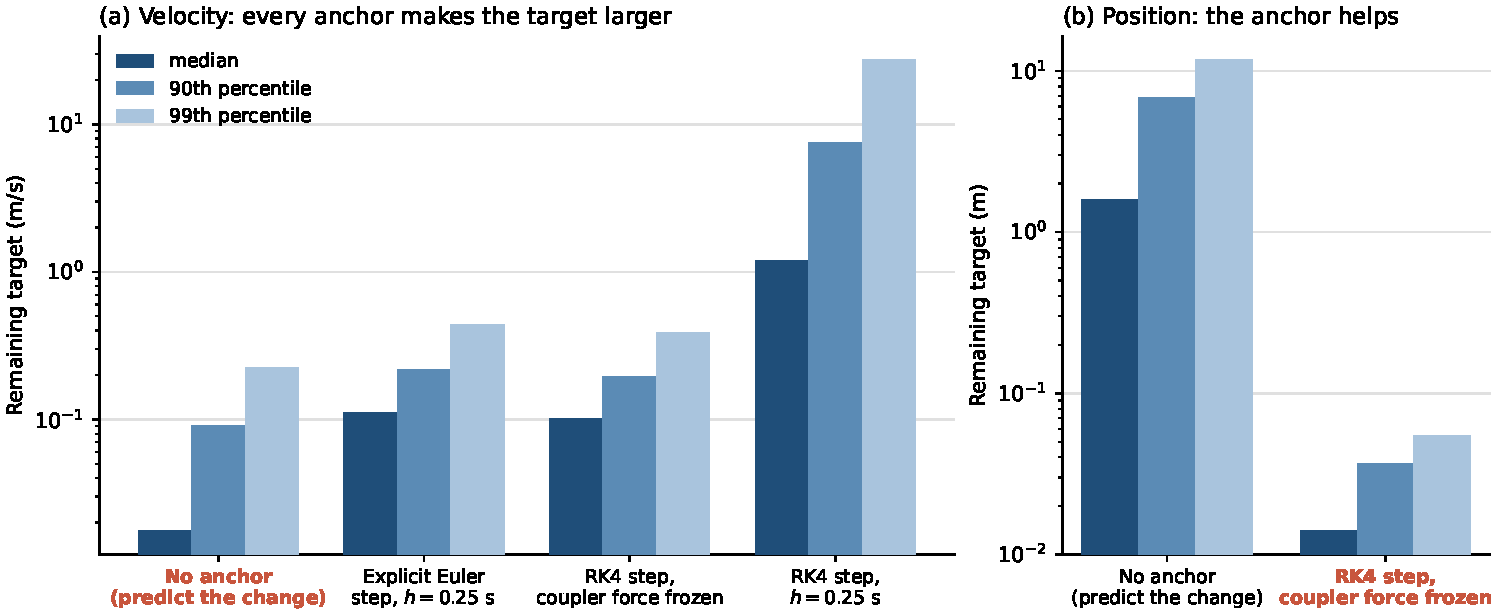
\includegraphics[width=\textwidth]{figures/arch_anchor_comparison.pdf}
    \caption{The size of the remaining learning target under each anchor, on a logarithmic scale. (a) For velocity, every physics anchor leaves a larger target than predicting the change directly. (b) For position, anchoring on the physics reduces the target more than a hundredfold. The best choice in each panel is marked in red. Data from \cref{tab:arch_anchor_velocity,tab:arch_anchor_position}.}
    \label{fig:arch_anchor}
\end{figure}

Every physics anchor makes the velocity target larger, by a factor of about six at the median for the best of them. A single RK4 step at the full 0.25\,s diverges outright. The reason is stiffness. Each coupler is a stiff spring between two heavy vehicles, and the pair has a natural frequency $\omega = \sqrt{k\,(1/m_j + 1/m_{j+1})}$, where $k$ is the coupler stiffness and $m_j$, $m_{j+1}$ the two masses. \Cref{tab:arch_stiffness} gives its distribution over the sampled consists.

\begin{table}[htbp]
    \centering
    \begin{tabular}{lccc}
        \toprule
        Coupler branch & Median $\omega$ & 99th pct. $\omega$ & Shortest period \\
        \midrule
        Buff (compression) & 17.4\,rad/s & 29.8\,rad/s & 0.211\,s \\
        Draft (tension)    & 15.1\,rad/s & 25.8\,rad/s & 0.243\,s \\
        \bottomrule
    \end{tabular}
    \caption{Natural frequency of the two-vehicle coupler mode, over 60 sampled scenarios.}
    \label{tab:arch_stiffness}
\end{table}

An explicit integrator is stable only while $\omega h$ stays below a limit set by the method, about 2.8 for RK4. At $h = 0.25$\,s, $\omega h$ reaches 7.45. The instability disappears only at $h \le 0.05$\,s, where the 99th percentile of $\omega h$ is 1.49, and that is the limit that forces a neural ODE to five or more calls per stored step. Nor is this an occasional regime: couplers are outside their slack, and therefore stiff, 91.1\% of the time. Freezing the coupler force over the step breaks the feedback loop that causes divergence, but the result is still six times worse than no anchor, because a force held constant over 250\,ms is a poor estimate of its own average.

It is worth separating this from a related concern. A shortest period of 0.21\,s is below the 0.25\,s sampling interval, which would suggest the stored data miss the peaks of coupler force. They do not. Re-integrating six high-force scenarios at a 2\,ms step and comparing peak force against the same trace sampled at 0.25\,s, the peak was missed by 0.4\% at the median and 3.7\% at worst. The couplers are heavily damped, with a damping ratio of about 0.37, and the forces are driven slowly by the bulk motion of the train rather than ringing. The \emph{trajectory} is smooth and well sampled at 0.25\,s; it is the \emph{explicit integrator} that is unstable there. Stability depends on $\omega h$, not on how smooth the solution is.

For position the picture reverses (\cref{tab:arch_anchor_position} and \cref{fig:arch_anchor}(b)). The relation $\dot x = v$ holds exactly, and anchoring on it leaves a target 113 times smaller at the median. The stiffness lives entirely in the velocity equation.

\begin{table}[htbp]
    \centering
    \begin{tabular}{lccc}
        \toprule
        Anchor for position & Median & 90th pct. & 99th pct. \\
        \midrule
        None: predict the change directly    & 1.582 & 6.796 & 11.73 \\
        RK4 step with coupler force frozen    & \textbf{0.014} & \textbf{0.037} & \textbf{0.055} \\
        \bottomrule
    \end{tabular}
    \caption{Size of the remaining learning target for position under each anchor, in metres, on the same transitions as \cref{tab:arch_anchor_velocity}.}
    \label{tab:arch_anchor_position}
\end{table}

The conclusion is that the anchor must be chosen per channel, not globally. The next section does that.

\section{Channel by channel}
\label{sec:arch_channels}

Each vehicle carries four dynamic channels: position $x_i$, velocity $v_i$, and the brake and traction lag states $z_{\mathrm{brk},i}$ and $z_{\mathrm{trac},i}$. Each coupler carries its stretch $\delta_j$, the change in the gap between vehicles $j$ and $j+1$ relative to its nominal length. \Cref{fig:arch_channels} summarizes how each is advanced.

\begin{figure}[htbp]
    \centering
    \resizebox{\textwidth}{!}{% Which state channels the network produces and which are imposed, against a
% design that learns a correction on every channel.
% Used by fig:arch_channels in chapters/08_surrogate_architecture.tex.
\begin{tikzpicture}[
    font=\small,
    >={Stealth[length=2.2mm]},
    ch/.style={draw=black!60, fill=white, rounded corners=2pt, line width=0.6pt,
               text width=2.7cm, minimum height=0.95cm, align=center},
    how/.style={draw=#1, fill=#1!10, rounded corners=2pt, line width=0.8pt,
                minimum height=0.95cm, text width=6.9cm, align=left, font=\footnotesize,
                inner sep=4pt},
    old/.style={draw=archLearned, fill=archLearned!10, rounded corners=2pt, line width=0.8pt,
                minimum height=0.95cm, minimum width=3.3cm, align=center, font=\footnotesize},
    hdr/.style={font=\small\bfseries, align=center},
]
\def\dy{1.3}

% ---- headers -----------------------------------------------------------------
\node[hdr] at (0, 1.0) {State channel};
\node[hdr] at (4.15, 1.0) {Correction-based design};
\node[hdr] at (10.4, 1.0) {This design};

% ---- rows ------------------------------------------------------------------
\foreach \y/\name/\sym in {0/{Velocity}/{v_i}, 1/{Coupler stretch}/{\delta_j},
                          2/{Position}/{x_i}, 3/{Brake lag}/{z_{\mathrm{brk},i}},
                          4/{Traction lag}/{z_{\mathrm{trac},i}}} {
  \node[ch] (c\y) at (0, {-\y*\dy}) {\name\\[-2pt]\footnotesize $\sym$};
}

% correction-based column: everything carries a learned correction
\foreach \y in {0,2,3,4} {
  \node[old] (o\y) at (4.15, {-\y*\dy}) {physics $+$ learned correction};
}
\node[font=\footnotesize\itshape, text=black!55, align=center] (o1) at (4.15, {-1*\dy})
    {derived from positions};

% this design
\node[how=archLearned] (n0) at (10.4, 0)
    {\textbf{learned:} mean acceleration over the step,\\
     $v_{k+1} = v_k + h\,\bar a_i$};
\node[how=archLearned] (n1) at (10.4, {-1*\dy})
    {\textbf{imposed, plus a learned correction:}\\
     trapezoid on the closing rate, plus $c_j$};
\node[how=archImposed] (n2) at (10.4, {-2*\dy})
    {\textbf{imposed:} centroid by trapezoid,\\
     shape rebuilt from the stretches $\delta_j$};
\node[how=archImposed] (n3) at (10.4, {-3*\dy})
    {\textbf{imposed:} exact solution of $\dot z = (u - z)/\tau$};
\node[how=archImposed] (n4) at (10.4, {-4*\dy})
    {\textbf{imposed:} exact solution of $\dot z = (u - z)/\tau$};

\foreach \y in {0,...,4} {
  \draw[black!25, line width=0.5pt] (c\y.east) -- (o\y.west);
  \draw[black!25, line width=0.5pt] (o\y.east) -- (n\y.west);
}

% ---- footer: what the network outputs --------------------------------------
\node[font=\footnotesize, align=center, text=archLearned] at (4.15, {-4*\dy-1.05})
    {network output: a correction on\\every channel of every vehicle};
\node[font=\footnotesize, align=center, text=archLearned] at (10.4, {-4*\dy-1.05})
    {network output: one scalar per vehicle ($\bar a_i$)\\and one per coupler ($c_j$)};
\end{tikzpicture}
}
    \caption{How each state channel is advanced over one step. A design that corrects the physics would learn a correction on every channel (centre). Here two channels are imposed exactly, position is imposed apart from the coupler shape, and the network's output narrows to one scalar per vehicle and one per coupler (right).}
    \label{fig:arch_channels}
\end{figure}

\subsection{Actuator lags: imposed exactly}

The brake and traction lag states obey $\dot z = (u - z)/\tau$, where $u$ is the commanded value and $\tau$ the lag time constant (\cref{ch:refsim}). The command is known in advance and varies linearly between stored samples, so the equation can be solved exactly across the step. With $r = h/\tau$,
\begin{equation}
    z_{k+1} = e^{-r} z_k + u_k\left(1 - e^{-r}\right) + \left(u_{k+1} - u_k\right)\left[1 - \frac{\tau}{h}\left(1 - e^{-r}\right)\right] .
    \label{eq:arch_actuator_exact}
\end{equation}
This is not an approximation of the data generator; it is the generator's own actuator model, solved. Checked against 25 scenarios, it reproduces the stored lag states to within $3.6\times10^{-3}$\,N on a scale of $9.2\times10^{4}$\,N, which is the rounding of single-precision storage, and a hundred times more accurately than an Euler step of the same equation. Giving these channels to the network would ask it to learn a first-order lag it can simply be told.

\subsection{Velocity: the one learned quantity}

The network's node output is the mean acceleration of each vehicle over the step, and velocity follows by definition:
\begin{equation}
    \bar a_i = \frac{v_{i,k+1} - v_{i,k}}{h}, \qquad v_{i,k+1} = v_{i,k} + h\,\bar a_i .
    \label{eq:arch_velocity}
\end{equation}
The target is the \emph{mean} acceleration over the step, not the instantaneous acceleration at its start. The two differ exactly where the dynamics are stiff, which is why no physics anchor helps (\cref{sec:arch_anchor}).

\subsection{Position: imposed, except for the shape of the train}

With the velocities at both ends of the step known, the trapezoid rule $x_{k+1} = x_k + \tfrac{h}{2}(v_k + v_{k+1})$ is the natural way to advance position. \Cref{tab:arch_position_split} measures how well it does when given the \emph{true} velocities, split into the motion of the train as a whole and its shape.

\begin{table}[htbp]
    \centering
    \begin{tabular}{lccc}
        \toprule
        Quantity & Trapezoid error & No-change error & Ratio \\
        \midrule
        Absolute position $x_i$              & 29.6\,mm & 3.67\,m & 124 \\
        Coupler stretch $\delta_j$            & 42.8\,mm & 54.7\,mm & 1.3 \\
        Bulk motion (consist centroid)        & 0.7\,mm  & 3.67\,m  & 5,219 \\
        Shape about the centroid              & 29.2\,mm & 87.5\,mm & 3.0 \\
        \bottomrule
    \end{tabular}
    \caption{Largest per-step error of the trapezoid rule computed from true velocities, against predicting no change, over 30 training scenarios.}
    \label{tab:arch_position_split}
\end{table}

The trapezoid carries the bulk motion of the train almost exactly, to 0.7\,mm per step. It fails on the shape. The error in coupler stretch, 43\,mm, is 2.1 times the coupler's 20\,mm half-slack, so a scheme that derived stretch from trapezoid positions would put couplers on the wrong side of their slack at every step. The cause is again stiffness: within one step, adjacent vehicles complete close to a full oscillation against each other, and the endpoints of an oscillation do not determine its integral. The kinematic relation is therefore kept, and the network supplies a small correction for the part it cannot recover.

Where that correction lives turned out to matter. Positions are stored in single precision and run to about 15\,km, where the spacing between representable numbers is 0.98\,mm. The correction has a standard deviation of 0.75\,mm, so as a per-vehicle position target it is mostly rounding error: the ratio of signal to quantization is 0.77. A first model trained on that target learned nothing from it, which was the correct behaviour. The same physical quantity expressed as a coupler stretch, on a scale of about 66\,mm, has a signal-to-quantization ratio of about 117,700. The correction is therefore predicted per coupler, and the network's edge output $c_j$ is added to a trapezoid update of the stretch:
\begin{equation}
    \delta_{j,k+1} = \delta_{j,k} + \frac{h}{2}\left(\dot\delta_{j,k} + \dot\delta_{j,k+1}\right) + c_j,
    \qquad \dot\delta_j = v_j - v_{j+1} .
    \label{eq:arch_stretch}
\end{equation}
Absolute positions are rebuilt from the two parts the analysis separated: the centroid of the consist advanced by the trapezoid rule, which is accurate to 0.7\,mm, and the shape of the train given by the new stretches, walking back from the lead vehicle through $\delta_j + L_{0,j}$, where $L_{0,j}$ is the nominal coupler spacing. Absolute position is then needed only to look up grade, curvature and speed limit, which vary over metres, so its millimetre rounding does no harm there, while the geometry the coupler law reads is carried at full precision. This also explains a storage decision of \cref{sec:dataset_format}: the coupler stretch is stored even though it can in principle be computed from positions, and at the precision the model needs it cannot.

\subsection{What the division achieves}

Two of the four vehicle channels leave the network entirely, and a third is imposed apart from a small shape correction. What the network produces narrows from a correction on every channel of every vehicle to one scalar per vehicle, $\bar a_i$, and one per coupler, $c_j$. The model imposes more physics than a correction-based design would, not less; the physics is built into the structure of the step rather than added to the network's output. The complete update is
\begin{equation}
\begin{aligned}
    (\bar a_i,\ c_j) &= \mathrm{GNN}_\theta\bigl(\mathbf{s}_k,\ \boldsymbol{\delta}_k,\ u_k,\ u_{k+1},\ \mathcal{R}\bigr), \\
    v_{i,k+1} &= v_{i,k} + h\,\bar a_i, \\
    \delta_{j,k+1} &= \delta_{j,k} + \tfrac{h}{2}\bigl(\dot\delta_{j,k} + \dot\delta_{j,k+1}\bigr) + c_j, \\
    \bar x_{k+1} &= \bar x_k + \tfrac{h}{2}\bigl(\bar v_k + \bar v_{k+1}\bigr), \quad x_{i,k+1} \text{ from } \bar x_{k+1} \text{ and } \boldsymbol{\delta}_{k+1}, \\
    z_{k+1} &= \text{\cref{eq:arch_actuator_exact}},
\end{aligned}
\label{eq:arch_update}
\end{equation}
where $\bar x$ and $\bar v$ are the mean position and velocity over the consist. The rest of the chapter describes $\mathrm{GNN}_\theta$.

\section{The network}
\label{sec:arch_network}

The network follows the encode--process--decode pattern of graph network simulators \cite{sanchez2020gns}: each vehicle's and coupler's features are first mapped into a larger internal representation, information is then exchanged along the chain for a fixed number of rounds, and finally each vehicle's and coupler's representation is mapped to its output. \Cref{fig:arch_overview} shows the whole pipeline, including the reconstruction of \cref{eq:arch_update} and the loop by which a rollout feeds each predicted state back in as the next input.

\begin{figure}[htbp]
    \centering
    \resizebox{\textwidth}{!}{% Encode-process-decode pipeline of the chain graph network, and the step
% reconstruction that turns its two outputs into the next state.
% Used by fig:arch_overview in chapters/08_surrogate_architecture.tex.
\begin{tikzpicture}[
    font=\small,
    >={Stealth[length=2.2mm]},
    stage/.style={draw=#1, fill=archFill, rounded corners=2pt, line width=0.7pt,
                  minimum width=2.6cm, minimum height=1.05cm, align=center},
    stage/.default=black!60,
    sub/.style={font=\footnotesize, text=black!70},
    lbl/.style={font=\footnotesize\itshape, text=black!60, align=center},
    flow/.style={->, line width=0.7pt, draw=black!70},
    veh/.style={circle, draw=black!70, fill=white, inner sep=0pt, minimum size=4.2mm},
]

% ---- column 1: inputs -------------------------------------------------------
\node[stage=archInput, text width=3.2cm] (nin) at (0, 1.15)
    {Node features\\[-2pt]\footnotesize 17 per vehicle\\[-3pt]\scriptsize state, commands, route};
\node[stage=archInput, text width=3.2cm] (ein) at (0,-1.15)
    {Edge features\\[-2pt]\footnotesize 9 per coupler\\[-3pt]\scriptsize stretch, rate, force};
\node[lbl] at (0, 2.25) {Inputs at step $k$};

% ---- column 2: encoders -----------------------------------------------------
\node[stage] (nenc) at (3.2, 1.15) {Node encoder\\[-2pt]\footnotesize MLP, $17 \to 128$};
\node[stage] (eenc) at (3.2,-1.15) {Edge encoder\\[-2pt]\footnotesize MLP, $9 \to 128$};
\node[lbl] at (3.2, 2.25) {Encode};
\draw[flow] (nin) -- (nenc);
\draw[flow] (ein) -- (eenc);

% ---- column 3: processor ----------------------------------------------------
\node[draw=black!60, fill=archFill, rounded corners=2pt, line width=0.7pt,
      minimum width=3.3cm, minimum height=3.35cm] (proc) at (6.75,0) {};
\node[lbl] at (6.75, 2.25) {Process};
\begin{scope}[shift={(6.75,0.55)}]
  \foreach \i in {0,...,4} {
    \node[veh] (c\i) at ({-1.2+0.6*\i}, 0) {};
  }
  \foreach \i [evaluate=\i as \j using int(\i+1)] in {0,...,3} {
    \draw[line width=0.9pt, black!70] (c\i) -- (c\j);
    \node[rectangle, fill=black!70, minimum size=1.6mm, inner sep=0pt]
        at ($(c\i)!0.5!(c\j)$) {};
  }
\end{scope}
\node[font=\footnotesize, align=center] at (6.75,-0.55)
    {edge update, then\\node update};
\node[font=\footnotesize, align=center] at (6.75,-1.25)
    {$\times\,R = 5$ rounds};
\draw[flow] (nenc.east) -- (proc.west |- nenc.east);
\draw[flow] (eenc.east) -- (proc.west |- eenc.east);

% ---- column 4: decoders -----------------------------------------------------
\node[stage=archLearned] (ndec) at (10.3, 1.15)
    {Node head\\[-2pt]\footnotesize $\bar a_i$ per vehicle};
\node[stage=archLearned] (edec) at (10.3,-1.15)
    {Edge head\\[-2pt]\footnotesize $c_j$ per coupler};
\node[lbl] at (10.3, 2.25) {Decode};
\draw[flow] (proc.east |- ndec.west) -- (ndec);
\draw[flow] (proc.east |- edec.west) -- (edec);

% ---- column 5: step reconstruction ------------------------------------------
\node[draw=archImposed, fill=archFill, rounded corners=2pt, line width=0.7pt,
      align=left, inner sep=6pt, font=\footnotesize,
      minimum height=3.35cm, text width=4.25cm] (rec) at (14.55,0) {%
    $v_{k+1} = v_k + h\,\bar a$\\[4pt]
    $\delta_{k+1} = \delta_k + \tfrac{h}{2}\bigl(\dot\delta_k + \dot\delta_{k+1}\bigr) + c$\\[4pt]
    \mbox{$x_{k+1}$: centroid by trapezoid,}\\ \mbox{\phantom{$x_{k+1}$:} shape from $\delta_{k+1}$}\\[4pt]
    $z_{k+1}$: exact lag solution};
\node[lbl] at (14.55, 2.25) {Reconstruct};
\draw[flow] (ndec.east) -- (rec.west |- ndec.east);
\draw[flow] (edec.east) -- (rec.west |- edec.east);

% ---- output and rollout loop ------------------------------------------------
\node[stage=archImposed, minimum width=1.5cm, minimum height=0.8cm] (out)
    at (14.55,-2.85) {$\mathbf{s}_{k+1}$};
\draw[flow] (rec) -- (out);
\coordinate (lp) at (-1.95,-2.85);
\draw[line width=0.7pt, dashed, draw=black!55] (out.west) -- (lp) -- (lp |- nin.west);
\draw[flow, dashed, draw=black!55] (lp |- nin.west) -- (nin.west);
\draw[flow, dashed, draw=black!55] (lp |- ein.west) -- (ein.west);
\node[lbl, fill=white, inner sep=2pt] at (6.75,-2.85)
    {rollout: features rebuilt from $\mathbf{s}_{k+1}$ for the next step};

% ---- legend -----------------------------------------------------------------
\begin{scope}[shift={(4.3,-3.75)}, font=\footnotesize]
  \draw[archInput, line width=1.4pt] (0,0) -- (0.45,0);
  \node[anchor=west] at (0.5,0) {inputs};
  \draw[archLearned, line width=1.4pt] (2.1,0) -- (2.55,0);
  \node[anchor=west] at (2.6,0) {learned by the network};
  \draw[archImposed, line width=1.4pt] (6.9,0) -- (7.35,0);
  \node[anchor=west] at (7.4,0) {imposed exactly};
\end{scope}
\end{tikzpicture}
}
    \caption{The surrogate as a whole. Node and edge features are encoded into 128-dimensional vectors, updated by five rounds of message passing along the chain, and decoded into the two learned outputs. The reconstruction step turns those into the next state exactly as in \cref{eq:arch_update}. In a rollout the new state is fed back as the next input.}
    \label{fig:arch_overview}
\end{figure}

\subsection{The graph and its features}

The graph is the consist itself: one node per vehicle and one edge per coupler, joined in a chain. Unlike the particle and mesh systems for which graph network simulators were developed, this graph never changes during a run and needs no neighbour search. Its connectivity is given by the consist manifest.

Each node carries 17 input features: the vehicle's velocity and two lag states; the traction and brake commands at both the start and the end of the step (four values); the vehicle's seven constant parameters (mass, three Davis coefficients, whether it is powered, and its maximum traction and brake forces); and the grade, curvature and speed limit of the route sampled at the vehicle's current position. Absolute position is deliberately excluded. A chainage of 12\,km means nothing that transfers to another route, and what the physics actually reads at that position, the route fields, is supplied directly.

Each edge carries 9 input features: the coupler's stretch, its rate of change, and its force, followed by six constant parameters (nominal spacing, slack half-width, and stiffness and damping in draft and in buff). The coupler force is computed from the stretch and rate with the known coupler law of \cref{ch:refsim}. This hands the network the slack explicitly instead of making it rediscover the discontinuity from raw positions. It is not information leakage, because at inference the force is computed in exactly the same way from the stretch the rollout carries. It is one more place where known physics enters as structure: the network is told the instantaneous force and must learn what it averages to over the step.

All features are standardized, each shifted by its mean and divided by its standard deviation over the training split, so that quantities measured in newtons, kilograms and metres per second enter on comparable scales. The two targets are standardized the same way.

\subsection{Encoding}

Two MLPs of the form of \cref{eq:arch_mlp}, one for nodes and one for edges, map the input features into 128-dimensional vectors, written $n_i$ for vehicle $i$ and $e_j$ for coupler $j$. These are the network's internal representation of each vehicle and coupler. They have no fixed physical meaning; training decides what each dimension encodes. The encoding lets the network describe the state in whatever combination of the inputs turns out to be useful, rather than in the units they arrive in.

\subsection{Message passing}

The core of the network is message passing \cite{battaglia2016interaction,gilmer2017mpnn}. In each of $R$ rounds, every coupler first updates its vector from its own vector and those of the two vehicles it joins, and every vehicle then updates its vector from its own and those of the two couplers attached to it:
\begin{align}
    e_j &\leftarrow e_j + \mathrm{LN}\bigl(\phi_e^{(r)}\bigl[\,e_j,\ n_j,\ n_{j+1}\,\bigr]\bigr), \label{eq:arch_edge_update} \\
    n_i &\leftarrow n_i + \mathrm{LN}\bigl(\phi_n^{(r)}\bigl[\,n_i,\ e_{i-1},\ e_i\,\bigr]\bigr), \label{eq:arch_node_update}
\end{align}
where square brackets denote concatenation of vectors, $\phi_e^{(r)}$ and $\phi_n^{(r)}$ are MLPs, and LN is layer normalization. \Cref{fig:arch_message_passing} shows one round.

\begin{figure}[htbp]
    \centering
    \resizebox{\textwidth}{!}{% One round of message passing on the consist chain: (a) the edge update,
% (b) the node update, (c) the end vehicles, (d) the update block itself.
% Used by fig:arch_message_passing in chapters/08_surrogate_architecture.tex.
\begin{tikzpicture}[
    font=\small,
    >={Stealth[length=2mm]},
    veh/.style={circle, draw=black!70, fill=white, line width=0.7pt,
                inner sep=0pt, minimum size=8.5mm, font=\footnotesize},
    vehhot/.style={veh, draw=archLearned, fill=archLearned!12, line width=1.1pt},
    cpl/.style={rectangle, draw=black!70, fill=black!70, inner sep=0pt, minimum size=2.4mm},
    cplhot/.style={rectangle, draw=archLearned, fill=archLearned, inner sep=0pt, minimum size=3.2mm},
    msg/.style={->, line width=0.9pt, draw=archLearned},
    panel/.style={font=\small\bfseries, anchor=west},
    note/.style={font=\footnotesize\itshape, text=black!60, align=center},
    blk/.style={draw=black!60, fill=archFill, rounded corners=2pt, line width=0.6pt,
                minimum height=0.85cm, align=center, font=\footnotesize},
]

% ============ (a) edge update ================================================
\begin{scope}[shift={(0,0)}]
  \node[panel] at (-0.5,1.5) {(a) Edge update};
  \node[veh]    (a0) at (0,0)   {$n_{j-1}$};
  \node[vehhot] (a1) at (2.1,0) {$n_{j}$};
  \node[vehhot] (a2) at (4.2,0) {$n_{j+1}$};
  \node[veh]    (a3) at (6.3,0) {$n_{j+2}$};
  \draw[line width=0.9pt, black!60] (a0) -- (a1) (a2) -- (a3);
  \draw[line width=1.2pt, archLearned] (a1) -- (a2);
  \node[cpl] at ($(a0)!0.5!(a1)$) {};
  \node[cplhot] (ej) at ($(a1)!0.5!(a2)$) {};
  \node[cpl] at ($(a2)!0.5!(a3)$) {};
  \node[font=\footnotesize, text=archLearned] at ($(ej)+(0,-0.45)$) {$e_j$};
  \draw[msg] (a1.north) to[bend left=45] (ej.north west);
  \draw[msg] (a2.north) to[bend right=45] (ej.north east);
  \node[font=\footnotesize] at (3.15,-1.25)
    {$e_j \leftarrow e_j + \mathrm{LN}\bigl(\phi_e^{(r)}[\,e_j,\ n_j,\ n_{j+1}\,]\bigr)$};
  \node[note] at (3.15,-1.8) {each coupler reads the two vehicles it joins};
\end{scope}

% ============ (b) node update ================================================
\begin{scope}[shift={(9.3,0)}]
  \node[panel] at (-0.5,1.5) {(b) Node update};
  \node[veh]    (b0) at (0,0)   {$n_{i-1}$};
  \node[vehhot] (b1) at (3.0,0) {$n_{i}$};
  \node[veh]    (b2) at (6.0,0) {$n_{i+1}$};
  \draw[line width=1.2pt, archLearned] (b0) -- (b1) -- (b2);
  \node[cplhot] (el) at ($(b0)!0.5!(b1)$) {};
  \node[cplhot] (er) at ($(b1)!0.5!(b2)$) {};
  \node[font=\footnotesize, text=archLearned] at ($(el)+(0,-0.45)$) {$e_{i-1}$};
  \node[font=\footnotesize, text=archLearned] at ($(er)+(0,-0.45)$) {$e_i$};
  \draw[msg] (el.north) to[bend left=45]
      node[pos=0.45, above, font=\scriptsize, text=black!70] {from ahead} (b1.north west);
  \draw[msg] (er.north) to[bend right=45]
      node[pos=0.45, above, font=\scriptsize, text=black!70] {from behind} (b1.north east);
  \node[font=\footnotesize] at (3.0,-1.25)
    {$n_i \leftarrow n_i + \mathrm{LN}\bigl(\phi_n^{(r)}[\,n_i,\ e_{i-1},\ e_i\,]\bigr)$};
  \node[note] at (3.0,-1.8) {the two messages are kept separate, not summed};
\end{scope}

% ============ (c) the end vehicles ===========================================
\begin{scope}[shift={(4.6,-4.4)}]
  \node[panel] at (-0.5,1.5) {(c) The ends of the train};
  \node[rectangle, draw=black!50, dashed, fill=white, minimum size=3.2mm, inner sep=0pt]
      (ghost) at (0.5,0) {};
  \node[font=\footnotesize, text=black!60] at (0.5,-0.45) {$\mathbf{0}$};
  \node[vehhot] (c0) at (2.1,0) {$n_0$};
  \node[veh] (c1) at (4.2,0) {$n_1$};
  \node[veh] (c2) at (6.3,0) {$n_2$};
  \draw[line width=0.9pt, black!40, dashed] (-0.1,0) -- (ghost.west) (ghost.east) -- (c0.west);
  \draw[line width=0.9pt, black!60] (c0) -- (c1) -- (c2);
  \node[cplhot] (ce0) at ($(c0)!0.5!(c1)$) {};
  \node[cpl] at ($(c1)!0.5!(c2)$) {};
  \node[font=\footnotesize, text=archLearned] at ($(ce0)+(0,-0.45)$) {$e_0$};
  \draw[msg, draw=black!45, dashed] (ghost.north) to[bend left=45] (c0.north west);
  \draw[msg] (ce0.north) to[bend right=45] (c0.north east);
  \node[note, text width=6.8cm] at (3.15,-1.45)
    {The lead vehicle has no coupler ahead of it. A zero vector stands in
     for the missing message, as a zero force does in the force balance.};
\end{scope}

% ============ (d) the update block ===========================================
\begin{scope}[shift={(0,-9.7)}]
  \node[panel] at (-0.5,2.2) {(d) Inside one update, $\phi^{(r)}$};
  \node[font=\footnotesize, align=right, anchor=east] (cur) at (1.2,0)
      {current state\\$e_j$ or $n_i$};
  \node[blk, minimum width=2.0cm] (cat) at (3.4,0) {concatenate\\[-2pt]\scriptsize $3\times128$};
  \node[blk, minimum width=1.9cm] (l1)  at (6.0,0) {Linear\\[-2pt]\scriptsize $384\to128$};
  \node[blk, minimum width=1.3cm] (act) at (8.2,0) {SiLU};
  \node[blk, minimum width=1.9cm] (l2)  at (10.4,0) {Linear\\[-2pt]\scriptsize $128\to128$};
  \node[blk, minimum width=1.9cm] (ln)  at (12.7,0) {LayerNorm};
  \node[circle, draw=black!70, line width=0.7pt, inner sep=0.5pt, font=\small] (add) at (14.4,0) {$+$};
  \node[font=\footnotesize, align=left, anchor=west] (upd) at (15.2,0)
      {updated state\\$e_j$ or $n_i$};
  \draw[->, line width=0.7pt, black!70] (cur.east) -- (cat.west);
  \foreach \a/\b in {cat/l1, l1/act, act/l2, l2/ln, ln/add, add/upd} {
    \draw[->, line width=0.7pt, black!70] (\a) -- (\b);
  }
  \draw[->, line width=0.7pt, black!70] (3.4,1.15)
      node[above, font=\footnotesize] {the two neighbours} -- (cat.north);
  \draw[->, line width=0.9pt, archImposed] (1.6,0) |- (14.4,-1.1) -- (add.south);
  \node[font=\scriptsize\itshape, text=archImposed, fill=white, inner sep=2pt]
      at (8.2,-1.1) {residual connection: the block learns a change to the current state, not a replacement};
\end{scope}
\end{tikzpicture}
}
    \caption{One round of message passing. (a) Each coupler updates from the two vehicles it joins. (b) Each vehicle then updates from the couplers ahead of and behind it, kept as separate inputs. (c) At the ends of the train a zero vector stands in for the missing coupler. (d) Each update is a two-layer MLP followed by layer normalization, added to the current vector through a residual connection.}
    \label{fig:arch_message_passing}
\end{figure}

The two updates mirror the physics directly. The edge update has the shape of the coupler law, $F_j = \phi_j(\delta_j, \dot\delta_j)$, which reads the two vehicles a coupler joins. The node update has the shape of the force balance $m_i\dot v_i = F_{\mathrm{ext},i} + F_{i-1} - F_i$, which combines the two coupler forces acting on a vehicle. Where the reference simulator evaluates a fixed spring law on each coupler and sums fixed forces at each vehicle, the network evaluates learned functions in the same places.

Several design choices within this pattern are specific to a train.

\paragraph{The same weights for every vehicle and coupler.} $\phi_e^{(r)}$ is applied to every coupler and $\phi_n^{(r)}$ to every vehicle, with the same weights. This is what makes the model independent of consist length: a 12-car and a 140-car train exercise exactly the same parameters, the second simply applies them more times. It is also the network's version of the fact that every vehicle obeys the same force balance, the structural assumption a plain MLP could not express (\cref{sec:arch_nn_primer}). Each round has its own pair of MLPs, so the five rounds can do different jobs, but within a round the weights are shared along the whole train.

\paragraph{Ordered messages, not a sum.} General message-passing networks combine the messages a node receives by summing or averaging them, since in a general graph a node's neighbours have no natural order. A vehicle's neighbours do: one coupler is ahead of it and one behind. The coupler law is also asymmetric, with different stiffness in draft and buff, so a vehicle pulled from ahead is in a different state from one pushed from behind, and a sum would discard that distinction. The two messages are therefore concatenated in a fixed order, front then rear, as \cref{eq:arch_node_update} shows.

\paragraph{The ends of the train.} The lead vehicle has no coupler ahead of it and the last has none behind. A zero vector stands in for the missing coupler, which matches the reference simulator's own convention that the end forces $F_{-1}$ and $F_{N-1}$ are zero (\cref{fig:arch_message_passing}(c)).

\paragraph{Residual connections and layer normalization.} Each update adds a learned change to the current vector rather than replacing it. This residual form \cite{he2016resnet} makes the identity, leaving a vector unchanged, the easiest thing for a round to do, so rounds that have nothing useful to add do no harm, and it keeps gradients well behaved through the stack of rounds during training. It also matches the nature of the task: each round refines a description of the train rather than rebuilding it. Layer normalization \cite{ba2016layernorm} rescales each update to a standard range using only that vector's own elements. Unlike batch normalization, it does not depend on the other examples in a batch or on the number of vehicles, so the network behaves the same on a short train as on a long one.

\paragraph{A smooth activation.} The nonlinearity $\sigma$ is the sigmoid-weighted linear unit, $\sigma(z) = z/(1 + e^{-z})$, often called SiLU \cite{elfwing2018silu}. Unlike the common rectified linear unit, which has a corner at zero, it is smooth everywhere. The surrogate will later be differentiated with respect to the control plan to choose driving commands, and a smooth network gives smooth gradients for that purpose.

\subsection{How many rounds: depth from the physics}

In one round, information moves one vehicle along the chain. After $r$ rounds a vehicle's vector depends on vehicles up to $r$ couplers away, and on nothing further (\cref{fig:arch_receptive_field}). The number of rounds is therefore the distance over which the network can relate cause and effect within one step. That distance has a physical counterpart: a disturbance travels along a train as a force wave through the couplers, at a speed set by coupler stiffness and vehicle mass. Measured from the consist parameters, the wave travels at 167 to 193\,m/s (median by coupler branch), against a car pitch of about 17\,m. In one 0.25\,s step it therefore reaches about three vehicles in each direction at the median and five at the 99th percentile.

\begin{figure}[htbp]
    \centering
    \resizebox{0.78\textwidth}{!}{% Receptive field of one vehicle after r rounds of message passing, against
% the distance a coupler force wave travels in one 0.25 s step.
% Used by fig:arch_receptive_field in chapters/08_surrogate_architecture.tex.
\begin{tikzpicture}[
    font=\small,
    dot/.style={circle, draw=black!45, fill=white, line width=0.5pt,
                inner sep=0pt, minimum size=3.6mm},
    reach/.style={dot, draw=archLearned!80, fill=archLearned!25},
    self/.style={dot, draw=archLearned, fill=archLearned, line width=0.8pt},
]
\def\sp{0.62}   % horizontal spacing between vehicles
\def\rh{0.62}   % vertical spacing between rounds
% rows: r = 0 (top) to r = 5 (bottom); vehicle offsets -7..7 around the target
\foreach \r in {0,...,5} {
  \node[anchor=east, font=\footnotesize] at ({-7*\sp-0.45}, {-\r*\rh})
      {$r = \r$};
  \draw[black!30, line width=0.5pt] ({-7*\sp}, {-\r*\rh}) -- ({7*\sp}, {-\r*\rh});
  \foreach \k in {-7,...,7} {
    \pgfmathtruncatemacro{\a}{abs(\k)}
    \ifnum\k=0
      \node[self] at ({\k*\sp}, {-\r*\rh}) {};
    \else\ifnum\a>\r
      \node[dot] at ({\k*\sp}, {-\r*\rh}) {};
    \else
      \node[reach] at ({\k*\sp}, {-\r*\rh}) {};
    \fi\fi
  }
}
\node[font=\footnotesize\itshape, text=black!60] at (0,0.45) {vehicle $i$};

% physical reach of one step
\pgfmathsetmacro{\yb}{-5*\rh-0.7}
\pgfmathsetmacro{\yc}{\yb-0.75}
\draw[archImposed, line width=2.4pt] ({-3*\sp}, \yb) -- ({3*\sp}, \yb);
\node[font=\footnotesize, text=archImposed, anchor=north] at (0, \yb-0.08)
    {force wave in 0.25\,s, median: about 3 vehicles each way};
\draw[archImposed!60, line width=2.4pt] ({-5*\sp}, \yc) -- ({5*\sp}, \yc);
\node[font=\footnotesize, text=archImposed!80, anchor=north] at (0, \yc-0.08)
    {99th percentile: about 5 vehicles each way};

\end{tikzpicture}
}
    \caption{Receptive field of vehicle $i$ after $r$ rounds of message passing. After $r$ rounds it has received information from vehicles up to $r$ couplers away, and no further. A coupler force wave travels 167--193\,m/s, about three vehicles each way in one 0.25\,s step at the median and five at the 99th percentile over a 17\,m car pitch, so five rounds cover the physical reach of one step.}
    \label{fig:arch_receptive_field}
\end{figure}

Five rounds cover that reach, and the network uses $R = 5$. The depth is fixed by physics rather than tuned, a line of argument also used for graph network simulators of structural dynamics \cite{lucchetti2025gnss}. It does not grow with the length of the train: a 150-car consist needs no more rounds than a 20-car one, because within one step no vehicle can be affected by anything further than the wave travels. Effects across the whole train build up over successive steps of a rollout, just as they do in the physical system.

\subsection{Decoding}

Two further MLPs read the final vectors. The node head maps each $n_i$ to the mean acceleration $\bar a_i$, and the edge head maps each $e_j$ to the stretch correction $c_j$. The two outputs are different quantities in different coordinates, one per vehicle and one per coupler, so they get separate decoders reading from the shared representation that message passing has built.

\subsection{Size, and independence from train length}

\Cref{tab:arch_params} counts the parameters. The network has 730,370 in total, and none of the counts depends on the number of vehicles. The same trained weights apply to a consist of any length, and the computation grows only linearly with it, one application of each MLP per vehicle or coupler per round. For comparison, the first layer alone of the plain MLP of \cref{sec:arch_nn_primer} would need about half a million weights, and would work only for trains of exactly 150 cars.

\begin{table}[htbp]
    \centering
    \begin{tabular}{lp{7.2cm}r}
        \toprule
        Component & Structure & Parameters \\
        \midrule
        Encoders        & two MLPs, $17 \to 128 \to 128$ and $9 \to 128 \to 128$ & 36,608 \\
        Message passing & five rounds, each an edge and a node MLP ($384 \to 128 \to 128$) and two layer normalizations & 660,480 \\
        Decoders        & two MLPs, $128 \to 128 \to 1$ & 33,282 \\
        \midrule
        Total                    &                                                  & 730,370 \\
        \bottomrule
    \end{tabular}
    \caption{Parameter count of the network. None of the counts depends on the number of vehicles.}
    \label{tab:arch_params}
\end{table}

\subsection{Implementation}

Because the graph is a chain, message passing needs no graph library. Every coupler reads its two vehicles by offsetting the vehicle array by one position, and every vehicle gathers its two couplers by padding the coupler array with a zero at one end or the other. This is the same pattern the GPU integrator uses to compute coupler forces (\cref{sec:gpu_port}), in the same batch-by-vehicle array layout. Training batches are drawn from one consist size at a time, so every batch is rectangular and needs no padding or masking, even though consist size ranges from 10 to 150. The model itself never sees the difference.

\section{Training objective}
\label{sec:arch_objective}

The network is trained to predict its two targets, the mean acceleration of \cref{eq:arch_velocity} and the stretch correction defined by \cref{eq:arch_stretch}, from a stored state. The loss is the sum of the mean squared errors of the two standardized outputs,
\begin{equation}
    \mathcal{L}(\theta) = \frac{1}{N}\sum_i \bigl(\hat a_i - \bar a_i\bigr)^2 + \frac{1}{N-1}\sum_j \bigl(\hat c_j - c_j\bigr)^2 ,
    \label{eq:arch_loss}
\end{equation}
with hats denoting predictions. Because both targets are standardized, this weights them equally relative to their own spread rather than by their physical magnitudes, which differ by orders of magnitude. The imposed channels contribute nothing: they are exact, so there is no error in them to fit. This is the concrete form of the objective of \cref{eq:training_loss}. Parameters are updated with the Adam optimizer \cite{kingma2015adam}, with a learning rate decaying from $10^{-3}$ along a cosine schedule and gradients clipped to a norm of 1. A model trained only to predict one step from true states does not remain stable when fed its own predictions; the techniques that make it stable over long rollouts are the subject of the training chapter.
% TODO: \cref the training chapter once it exists.

\section{Relation to graph network simulators}
\label{sec:arch_relation_gns}

The model belongs to the graph network simulator family and borrows its structure, its name, and its central idea that a learned step is advanced by a fixed update. It departs from the original in ways that follow from the problem. \Cref{tab:arch_gns_comparison} sets the two side by side.

\begin{table}[htbp]
    \centering
    \begin{tabular}{p{3.0cm}p{5.2cm}p{5.8cm}}
        \toprule
         & Graph network simulator \cite{sanchez2020gns} & This model \\
        \midrule
        Nodes and edges & particles; edges between particles within a radius & vehicles; edges are the couplers \\
        Graph & rebuilt at every step by neighbour search & fixed chain, given by the consist \\
        Combining messages & sum over neighbours & ordered concatenation, front and rear \\
        Network output & acceleration per particle & mean acceleration per vehicle and a stretch correction per coupler \\
        Update rule & fixed integrator on all channels & velocity from the output; position by trapezoid with learned shape; lag states exact \\
        Depth & tuned & set by force-wave travel in one step \\
        \bottomrule
    \end{tabular}
    \caption{The original graph network simulator and the model of this chapter.}
    \label{tab:arch_gns_comparison}
\end{table}

\section{Chapter summary}

The surrogate predicts one fixed 0.25\,s step, replacing fifty evaluations of the reference right-hand side with one network evaluation. A learned correction to the right-hand side was rejected because, against data generated by that right-hand side, the correction is identically zero, and a learned derivative because coupler stiffness would force at least five network calls per step between unsupervised states. Measurement showed that no physics anchor helps velocity, since the couplers are stiff at this step size, while the kinematic anchor helps position a hundredfold. The step is therefore built channel by channel: lag states exact, velocity learned as a mean acceleration, position by the trapezoid rule on the bulk motion with a learned correction to the shape of the train, predicted per coupler because only there does it survive single-precision storage.

The network that supplies those two outputs is a message-passing graph network on the consist chain: encoders into 128-dimensional vectors, five rounds of edge and node updates with residual connections and layer normalization, and one decoder for each output. Its weights are shared across every vehicle and every coupler, so its 730,370 parameters apply unchanged to a train of any length, and its depth is set by how far a force wave travels in one step rather than by tuning. The next chapter describes how it is trained to stay stable when run on its own predictions over hundreds of steps.
